\documentclass[11pt]{article}
\usepackage{epsf,amsmath,amsfonts,amsthm,graphicx,color}
%\usepackage{draftcopy}
\textwidth=7in
\textheight=9.0in
\hoffset=-1in
\voffset=-1in
\bibliographystyle{alpha}

\usepackage{amsthm, amsmath, amssymb, amsfonts, graphicx, graphics,epsfig, bbm, xcolor, hyperref,subfigure,float}


\newcommand{\xinnote}[1]{ {\textcolor{red}  {\mbox{**Xin:} #1}}}
\newcommand{\nichollsnote}[1]{ {\textcolor{yellow}  {\mbox{**Nicholls:} #1}}}
\newcommand{\hpra}{\frac{H_p^{(1)}(kr)}{H_p^{(1)}(ka)} }
\newcommand{\hprb}{\frac{H_p^{(1)}(kr)}{H_p^{(1)}(kb)} }
\newcommand{\diffhpn}{\frac{d_z^nH_p^{(1)}(ka)}{H_p^{(1)}(ka)} }
\newcommand{\diffhpnm}{\frac{d_z^{n-m}H_p^{(1)}(ka)}{H_p^{(1)}(ka)} }
\newcommand{\ep}{e^{ip\theta}}
\newcommand{\opD}{\mathcal{D}}
\newcommand{\jpra}{\frac{J_p(kr)}{J_p(ka)} }
\newcommand{\diffjpn}{\frac{d_z^nJ_p(ka)}{J_p(ka)} }
\newcommand{\diffjpnm}{\frac{d_z^{n-m}J_p(ka)}{J_p(ka)} }

\begin{document}
\noindent\textbf{\large Convergence Study---Numerical results}\\
\textbf{DNO, $G[U]$}
\begin{figure}[H]
	\centering
	\subfigure [DNO with $a=0.5$.] 
	{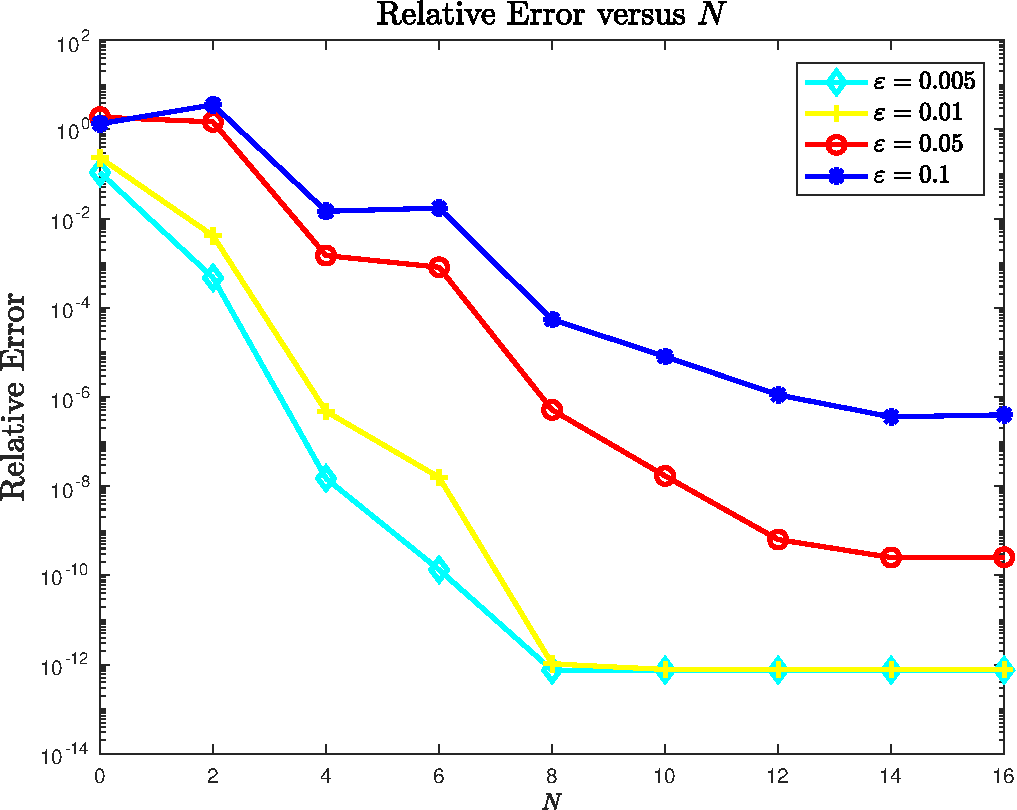
\includegraphics[width=0.4\textwidth]
		{fig_ErrrorVsN_DNO.pdf}}
	\quad
	\subfigure [DNO with $a=0.5$.] 
	{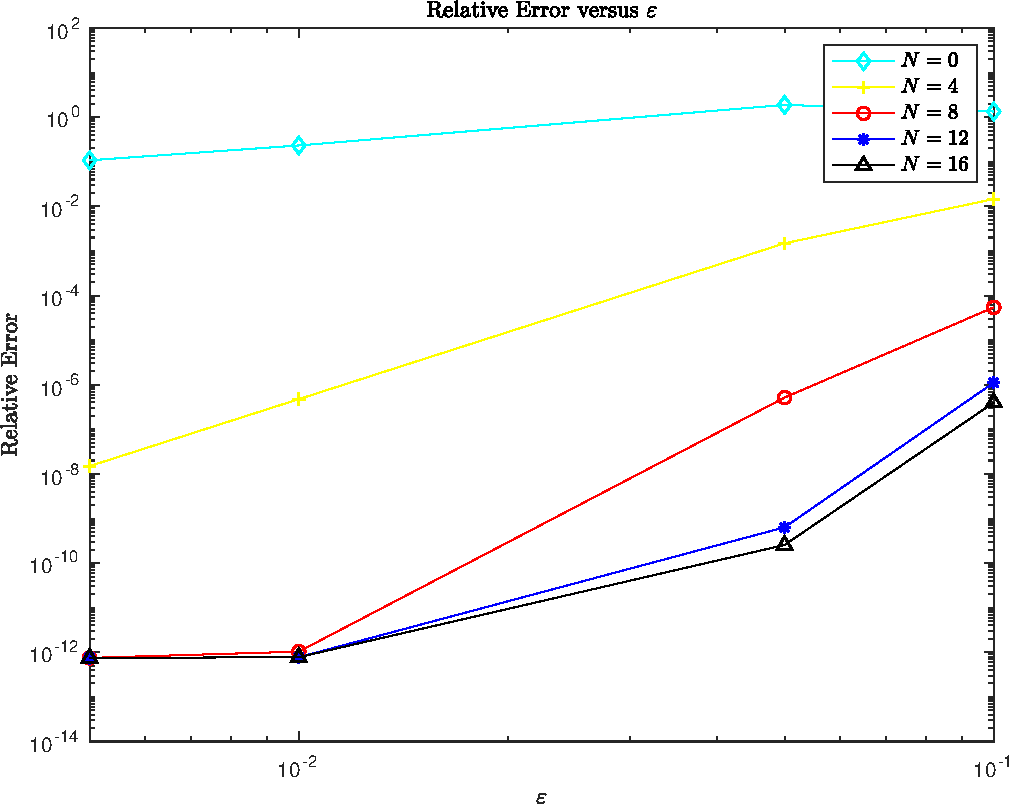
\includegraphics[width=0.4\textwidth]
		{fig_ErrrorVsEps_DNO.pdf}}
	\\
	\subfigure [DNO with $a=1-10^{12}$.] 
	{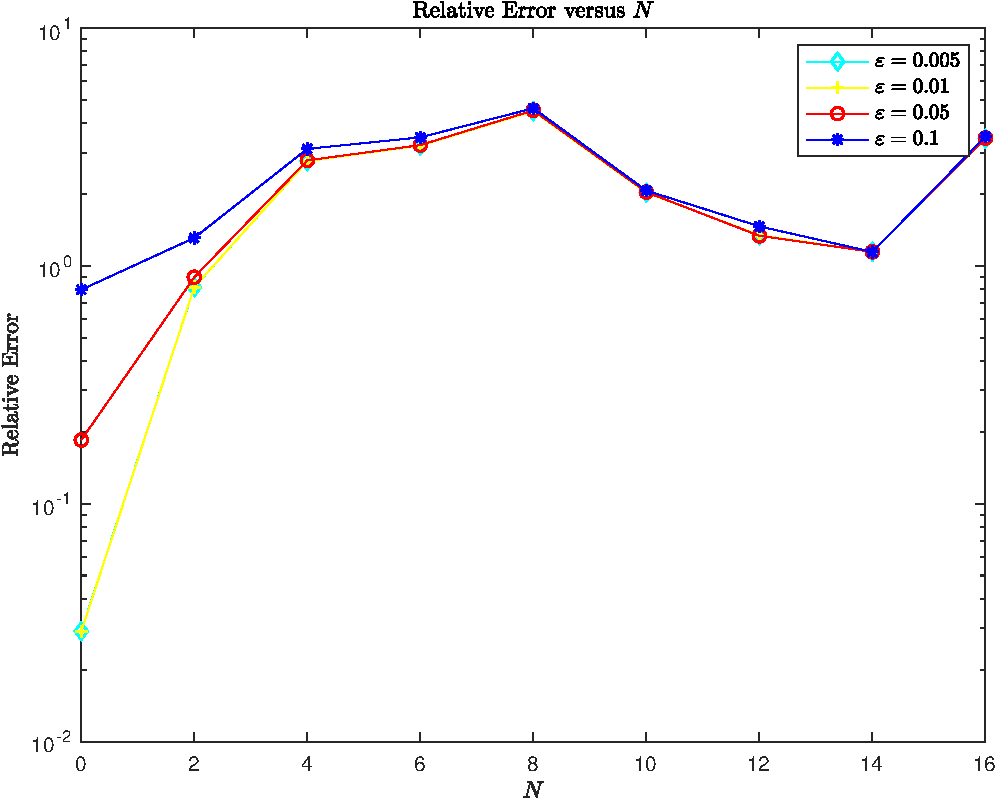
\includegraphics[width=0.4\textwidth]
		{fig_ErrrorVsN_DNO_sing12.pdf}}
	\quad
	\subfigure [DNO with $a=1-10^{12}$.] 
	{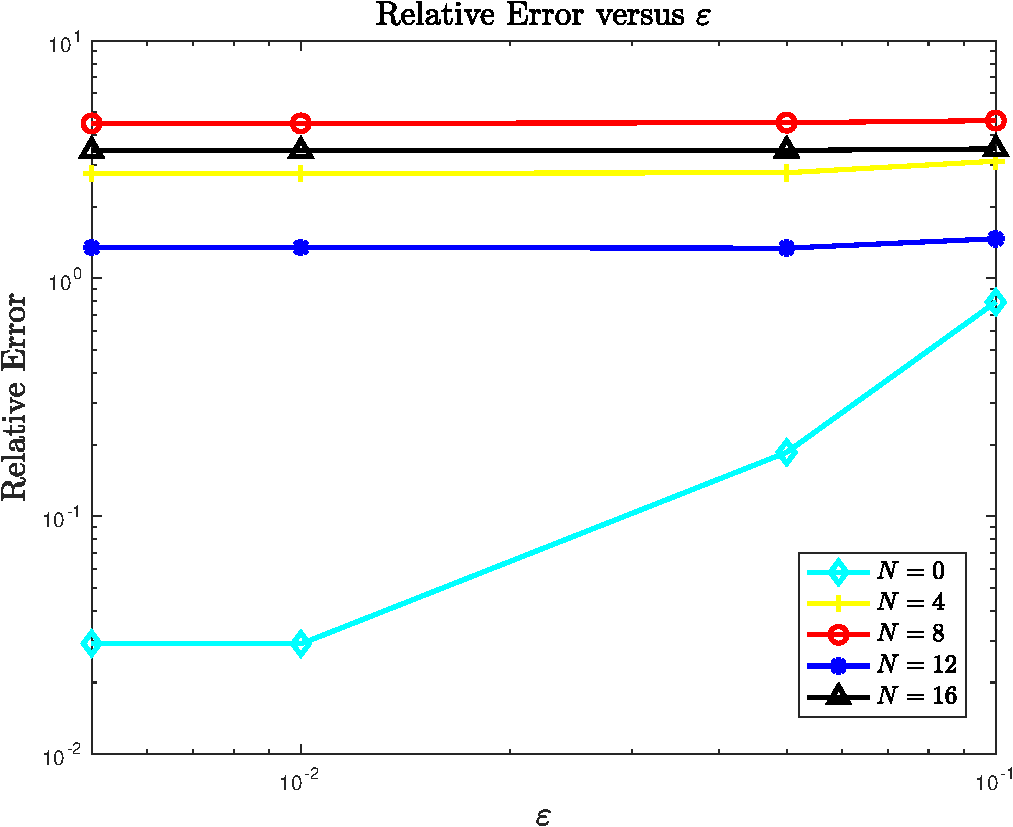
\includegraphics[width=0.4\textwidth]
		{fig_ErrrorVsEps_DNO_sing12.pdf}}
	\\
	\subfigure [DNO with $a=1-10^{16}$.] 
	{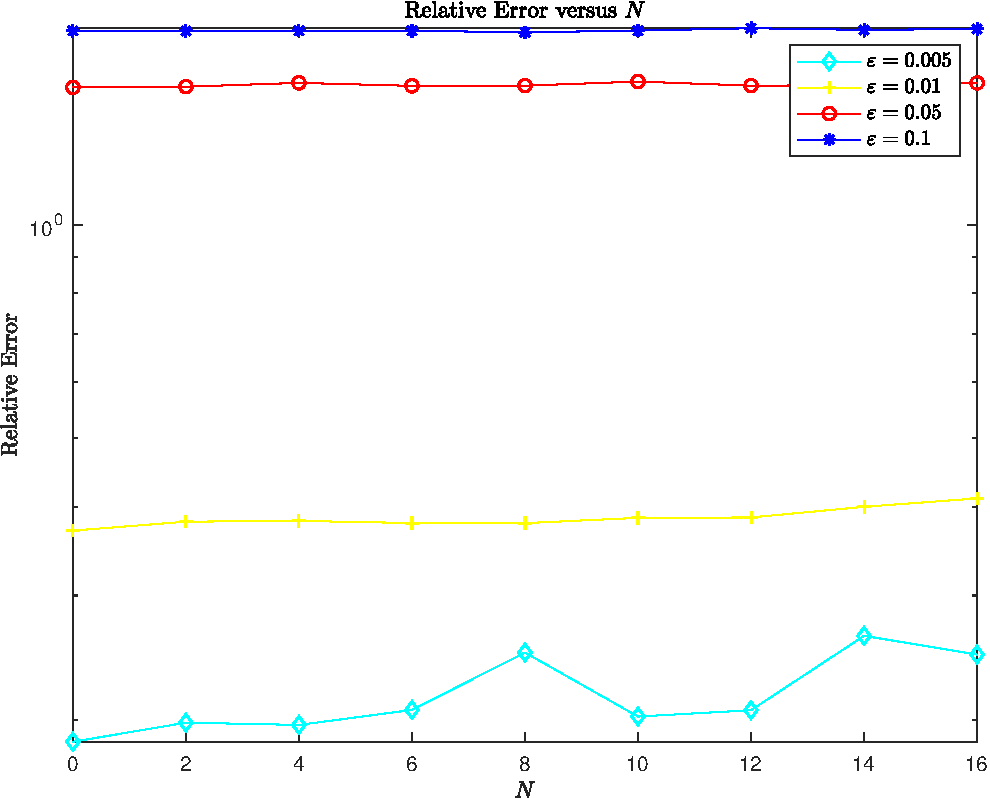
\includegraphics[width=0.4\textwidth]
		{fig_ErrrorVsN_DNO_sing16.pdf}}
	\quad
	\subfigure [DNO with $a=1-10^{16}$.] 
	{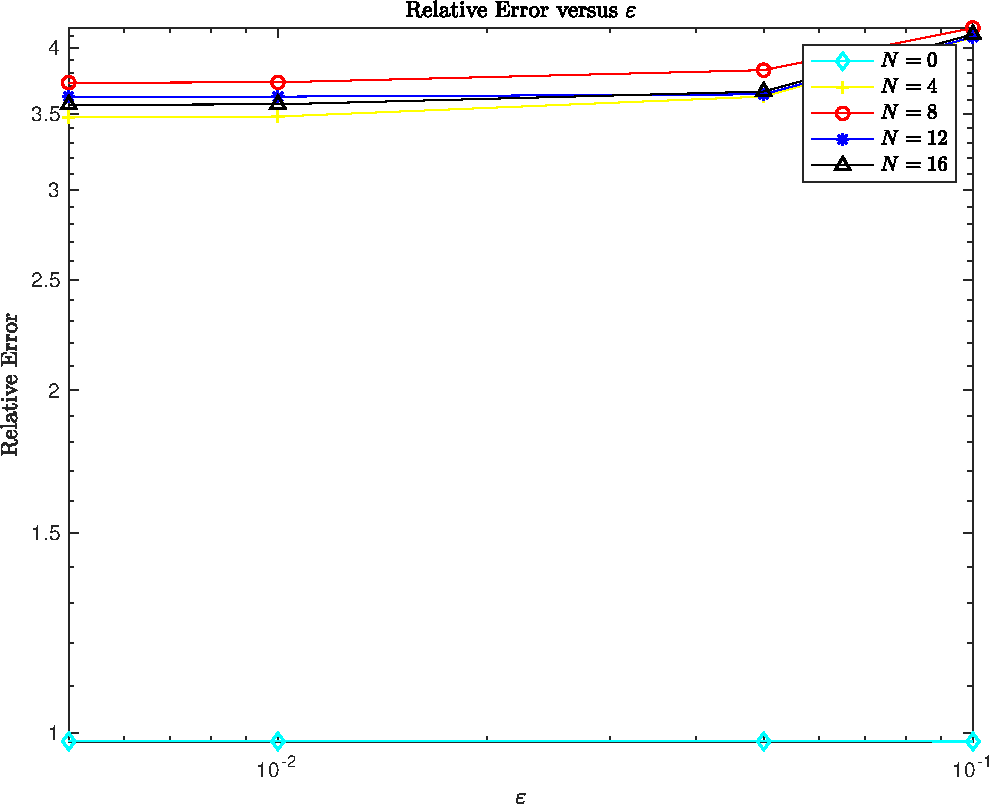
\includegraphics[width=0.4\textwidth]
		{fig_ErrrorVsEps_DNO_sing16.pdf}}
\end{figure}

\newpage
\textbf{IIO, $I[U]$}
\begin{figure}[H]
	\centering
	\subfigure [IIO with $a=0.5$.] 
	{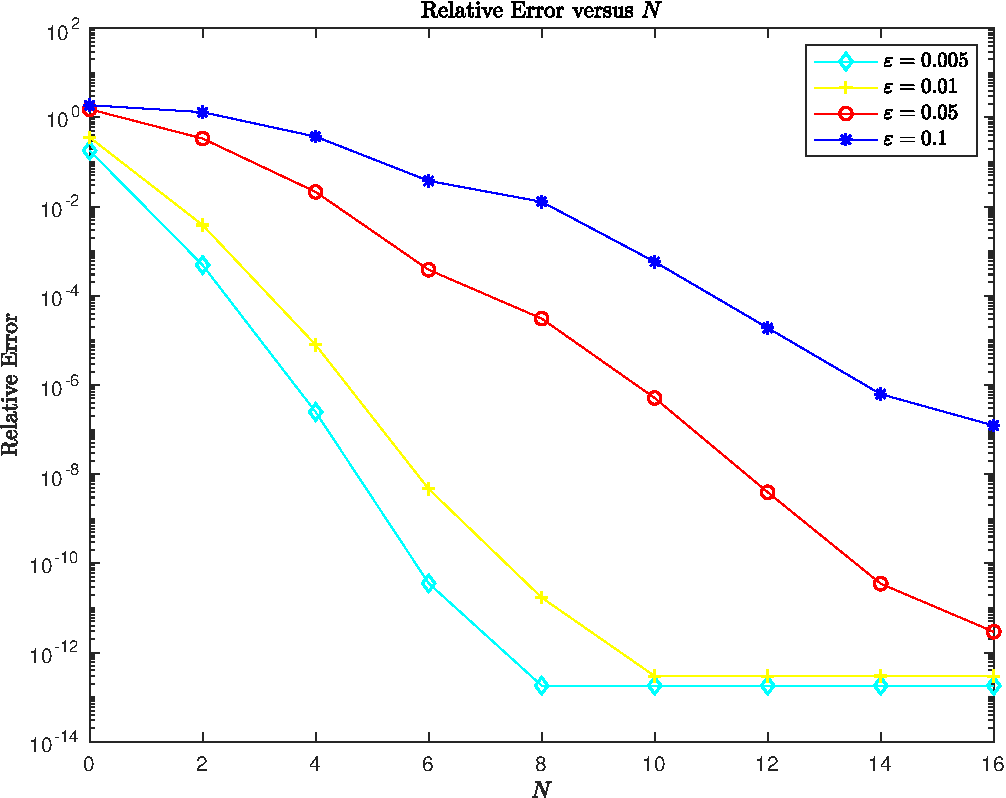
\includegraphics[width=0.4\textwidth]
		{fig_ErrrorVsN_IIO.pdf}}
	\quad
	\subfigure [IIO with $a=0.5$.] 
	{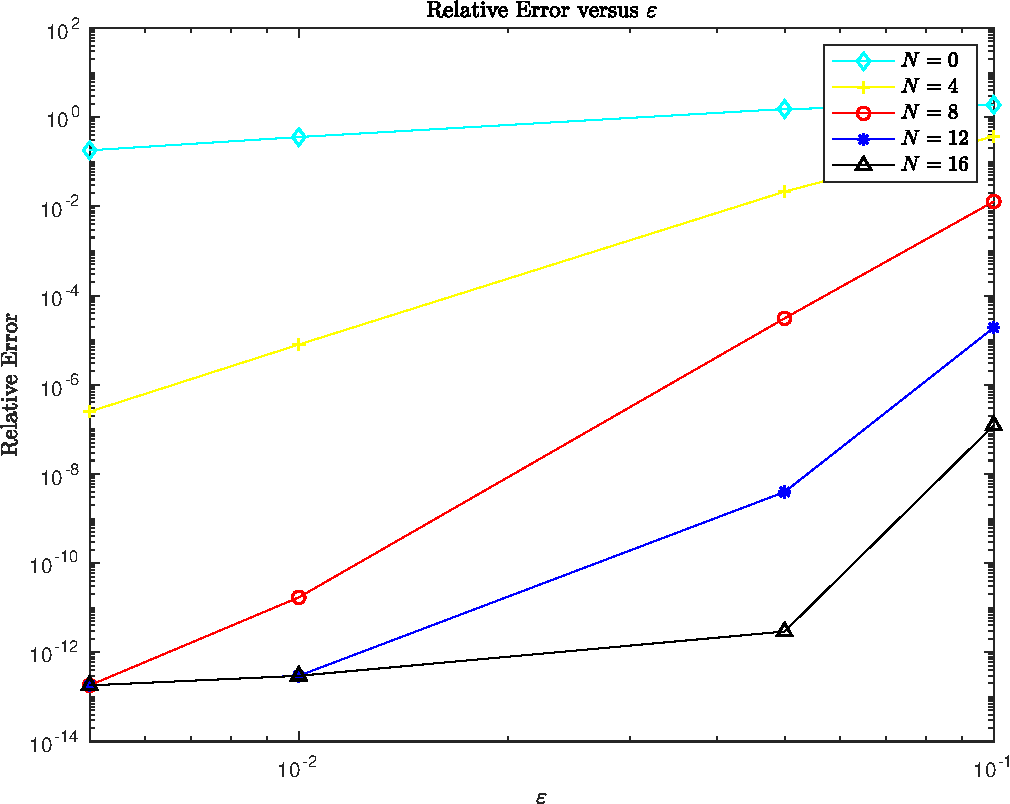
\includegraphics[width=0.4\textwidth]
		{fig_ErrrorVsEps_IIO.pdf}}
	\\
	\subfigure [IIO with $a=1-10^{12}$.] 
	{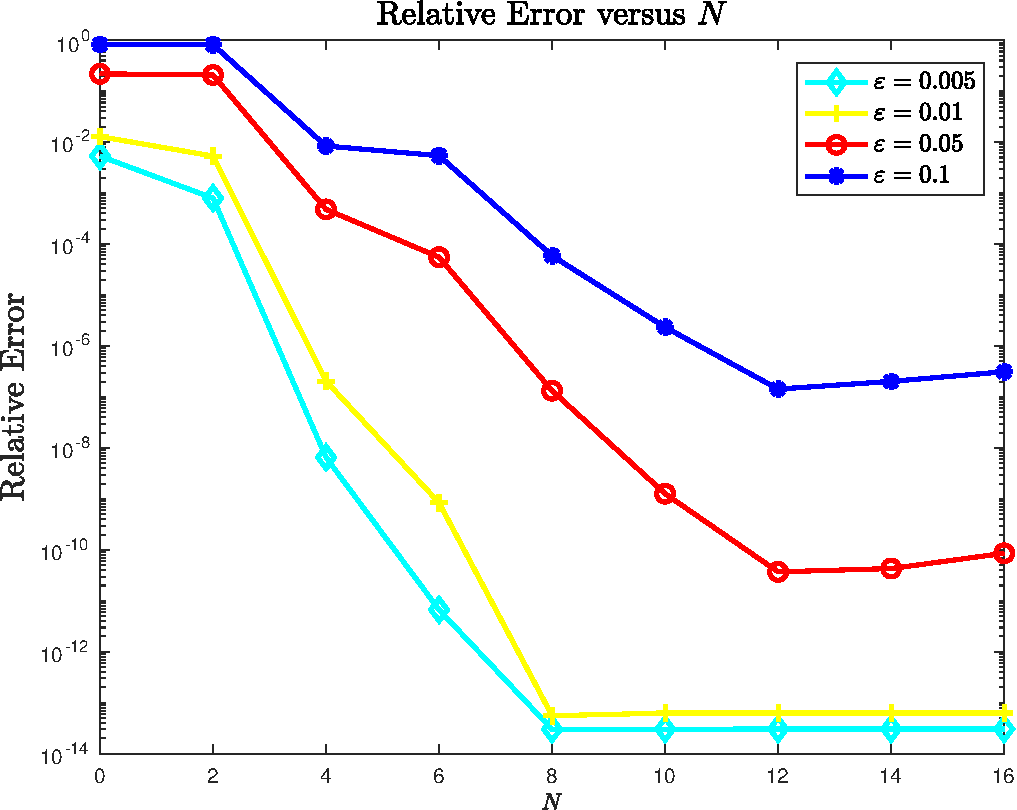
\includegraphics[width=0.4\textwidth]
		{fig_ErrrorVsN_IIO_sing12.pdf}}
	\quad
	\subfigure [IIO with $a=1-10^{12}$.] 
	{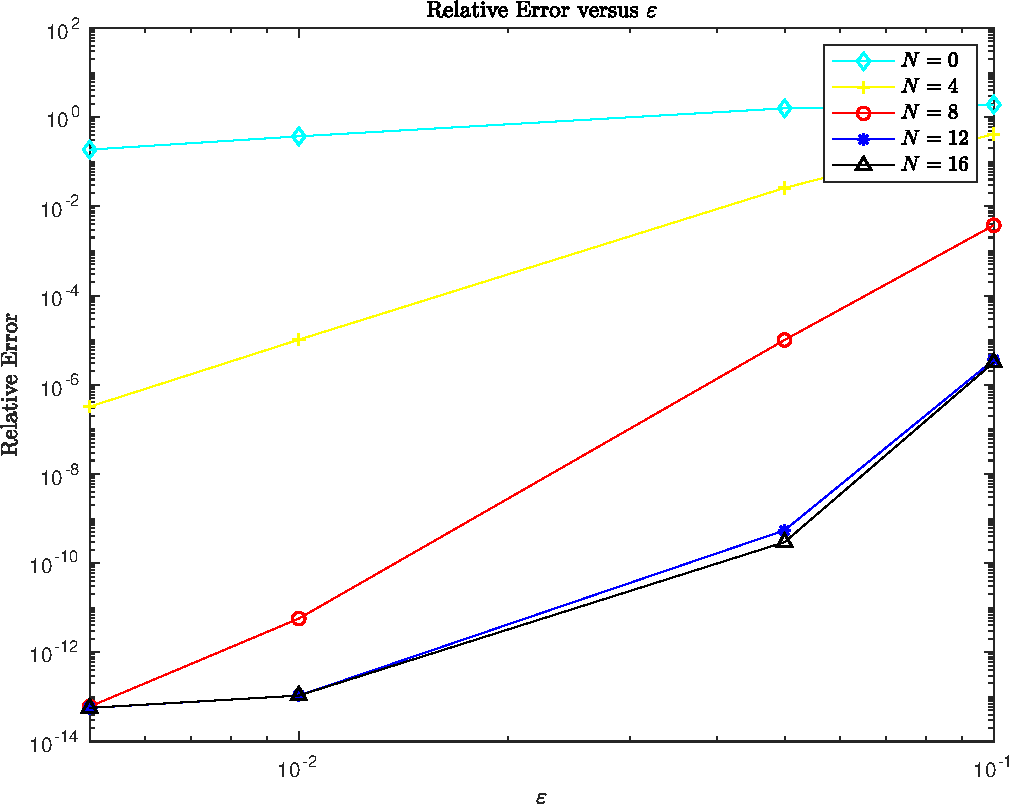
\includegraphics[width=0.4\textwidth]
		{fig_ErrrorVsEps_IIO_sing12.pdf}}
	\\
	\subfigure [IIO with $a=1-10^{16}$.] 
	{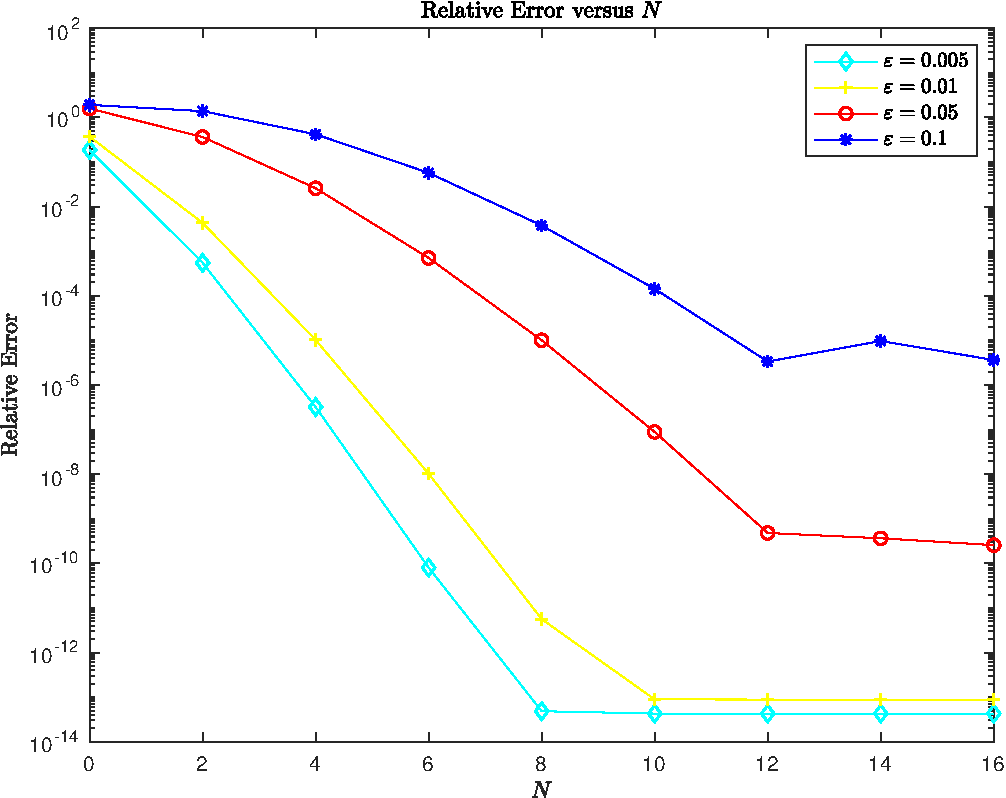
\includegraphics[width=0.4\textwidth]
		{fig_ErrrorVsN_IIO_sing16.pdf}}
	\quad
	\subfigure [IIO with $a=1-10^{16}$.] 
	{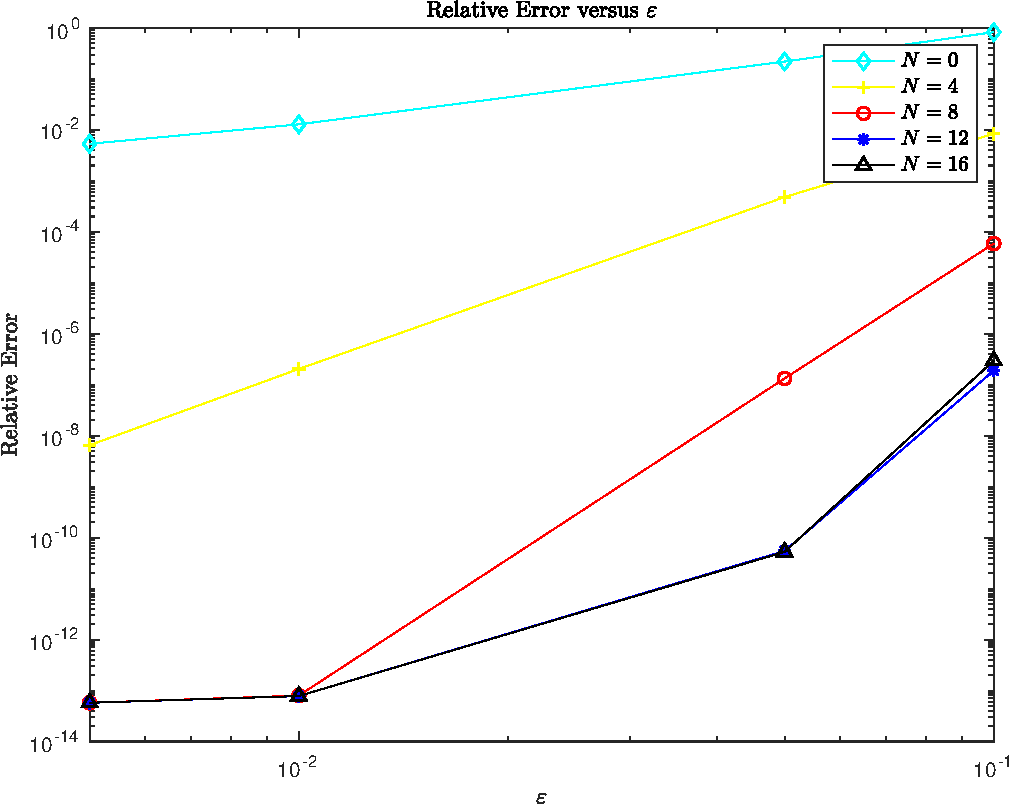
\includegraphics[width=0.4\textwidth]
		{fig_ErrrorVsEps_IIO_sing16.pdf}}
\end{figure}

\newpage
\textbf{new IIO, $I[U]$, relative error}
\begin{figure}[H]
	\centering
	\subfigure [new IIO with $a=0.5$.] 
	{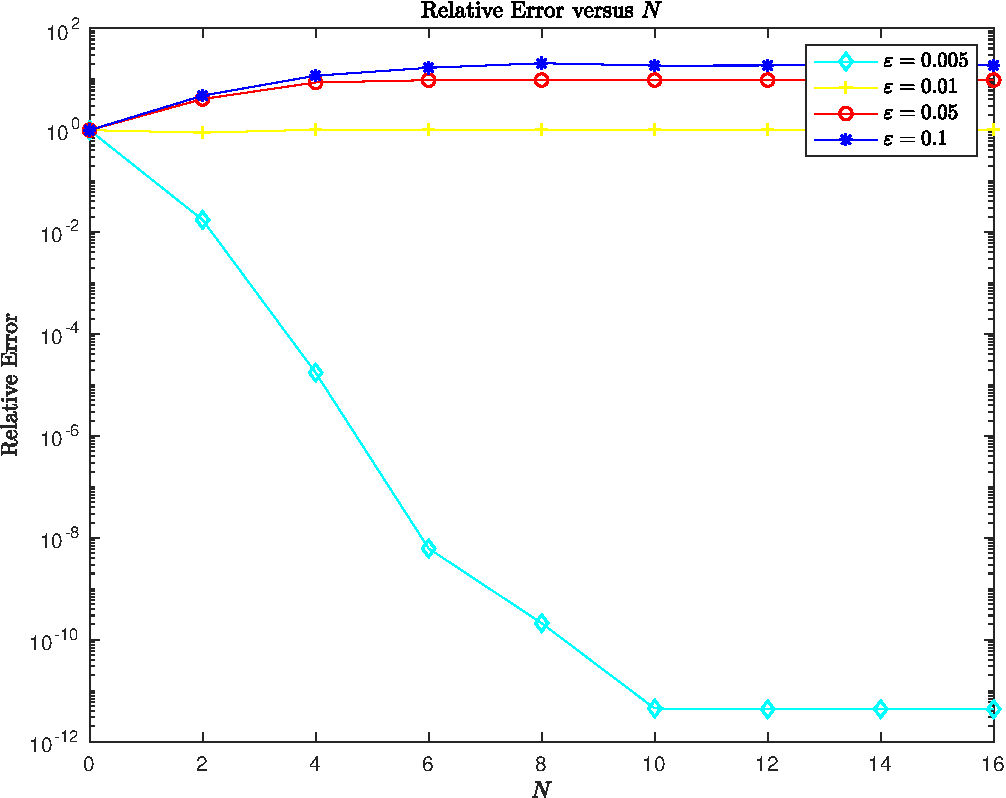
\includegraphics[width=0.4\textwidth]
		{fig_ErrrorVsN_IIO_new.pdf}}
	\quad
	\subfigure [new IIO with $a=0.5$.] 
	{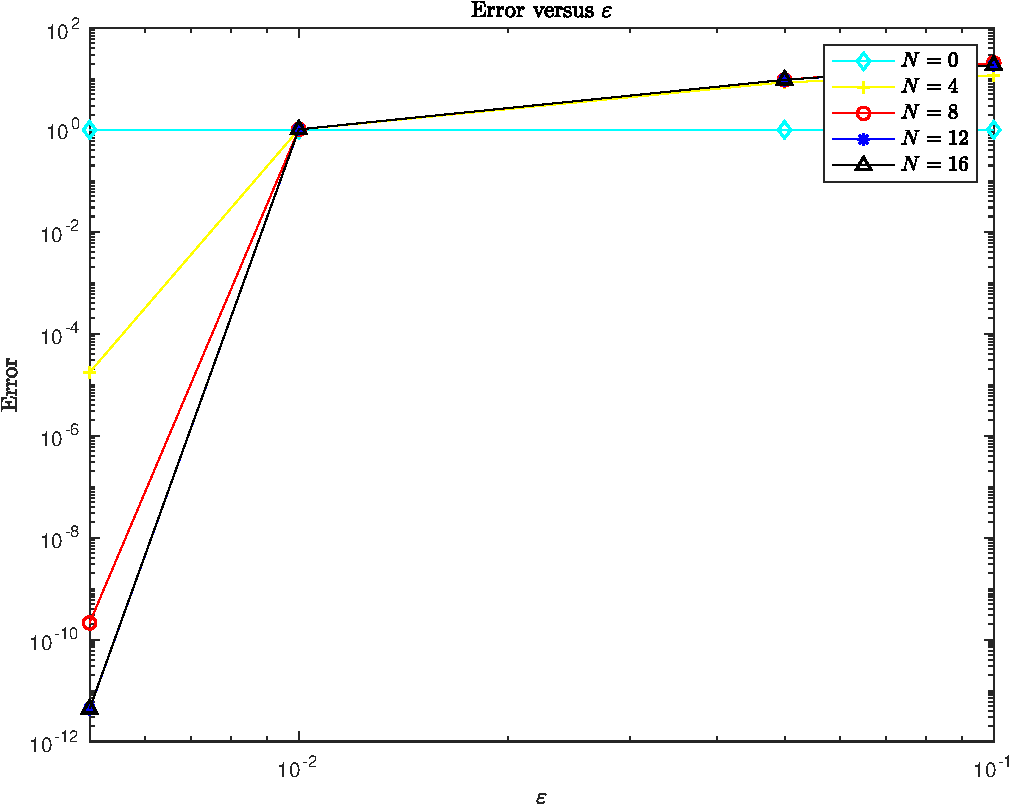
\includegraphics[width=0.4\textwidth]
		{fig_ErrrorVsEps_IIO_new.pdf}}
	\\
	\subfigure [new IIO with $a=1-10^{12}$.] 
	{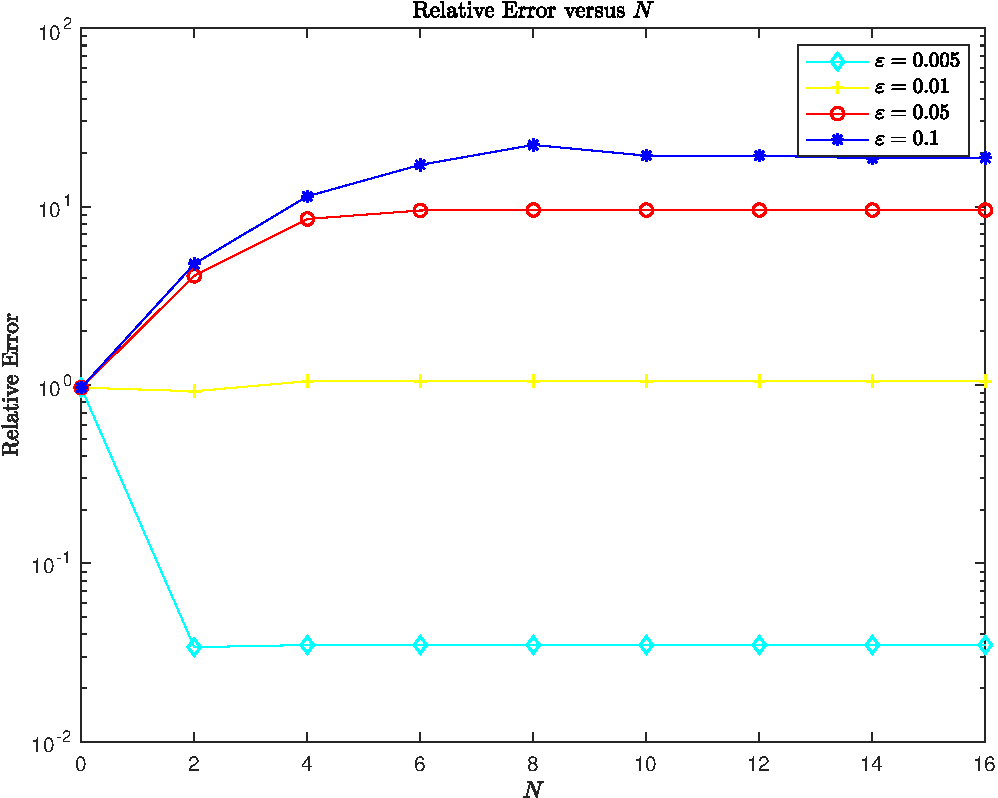
\includegraphics[width=0.4\textwidth]
		{fig_ErrrorVsN_IIO_new_sing12.pdf}}
	\quad
	\subfigure [new IIO with $a=1-10^{12}$.] 
	{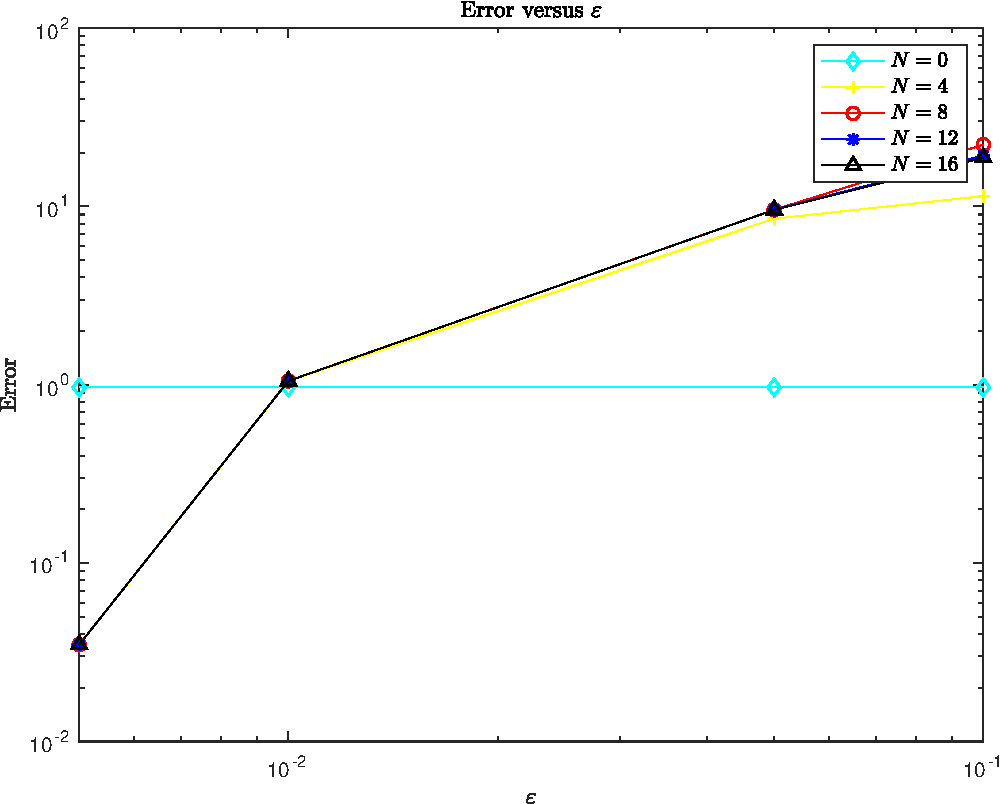
\includegraphics[width=0.4\textwidth]
		{fig_ErrrorVsEps_IIO_new_sing12.pdf}}
	\\
	\subfigure [new IIO with $a=1-10^{16}$.] 
	{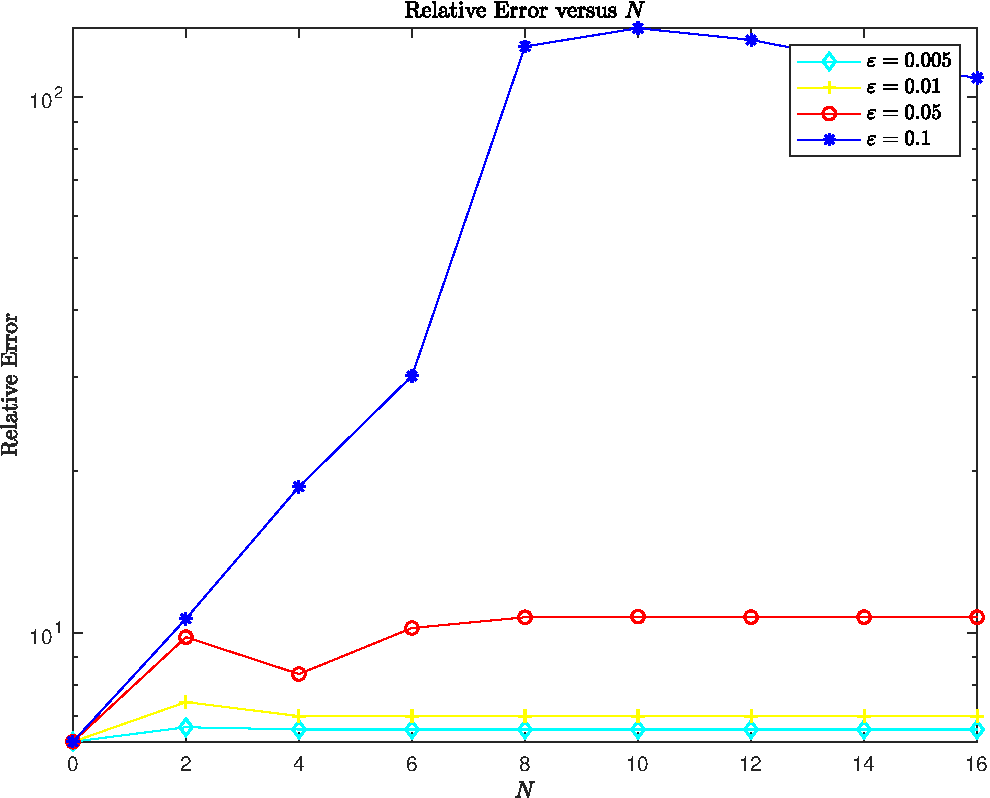
\includegraphics[width=0.4\textwidth]
		{fig_ErrrorVsN_IIO_new_sing16.pdf}}
	\quad
	\subfigure [new IIO with $a=1-10^{16}$.] 
	{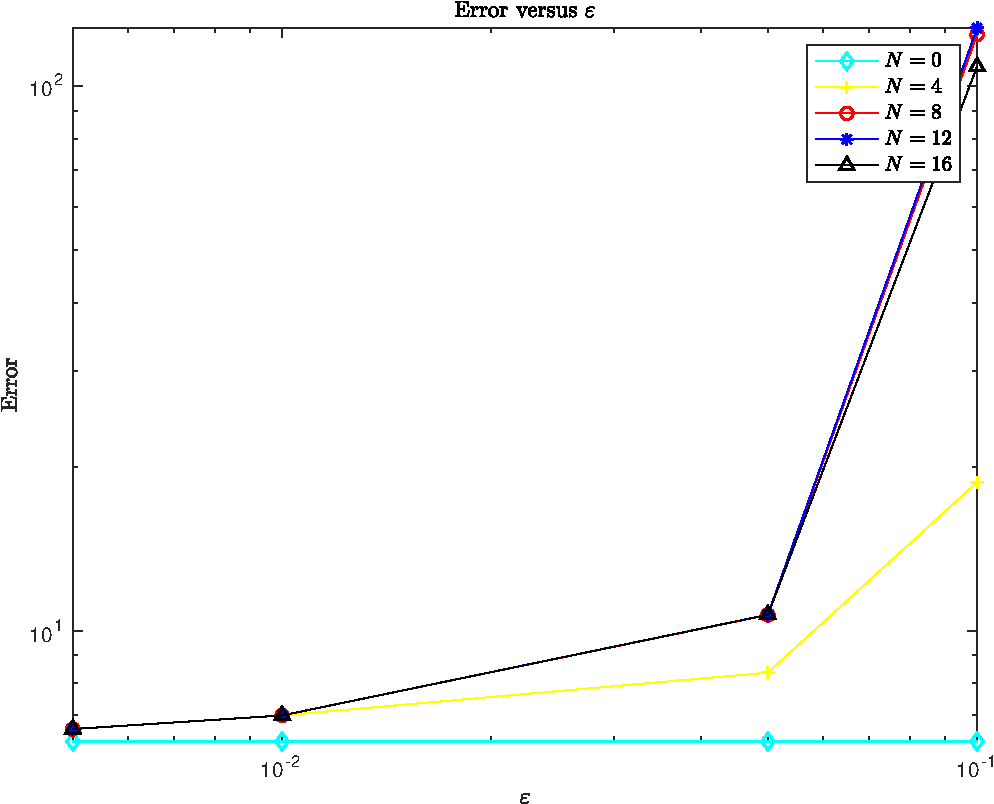
\includegraphics[width=0.4\textwidth]
		{fig_ErrrorVsEps_IIO_new_sing16.pdf}}
\end{figure}

\newpage
\textbf{new IIO, $I[U]$, absolute error}
\begin{figure}[H]
	\centering
	\subfigure [new IIO with $a=0.5$.] 
	{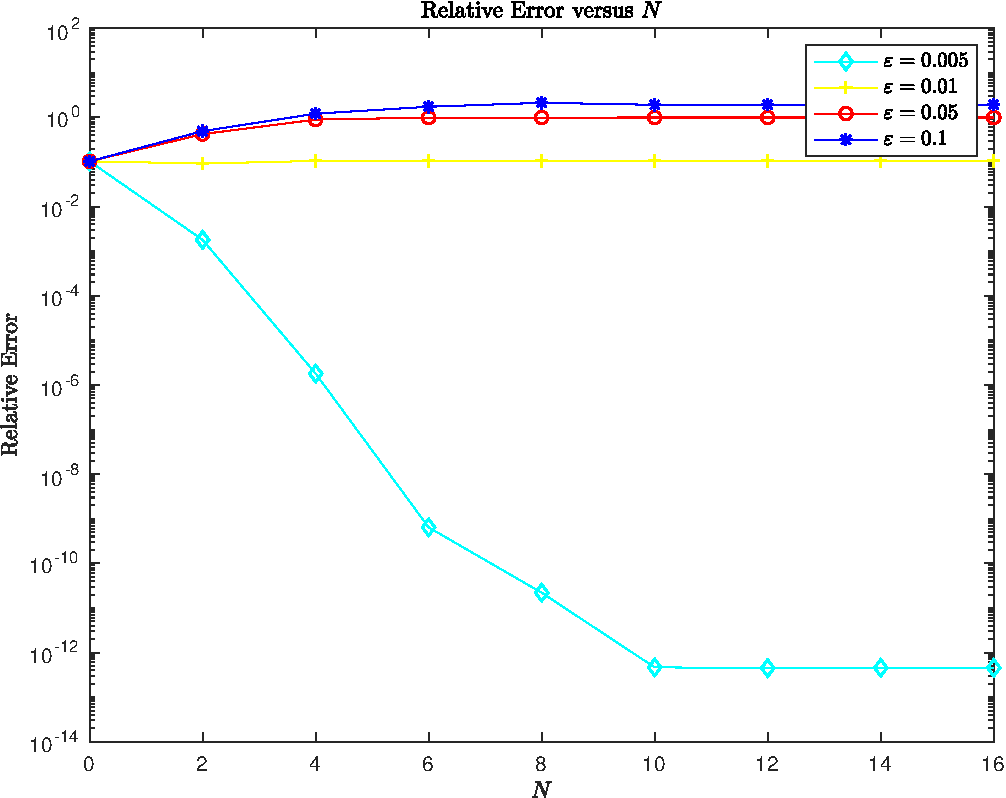
\includegraphics[width=0.4\textwidth]
		{fig_absErrrorVsN_IIO_new.pdf}}
	\quad
	\subfigure [new IIO with $a=0.5$.] 
	{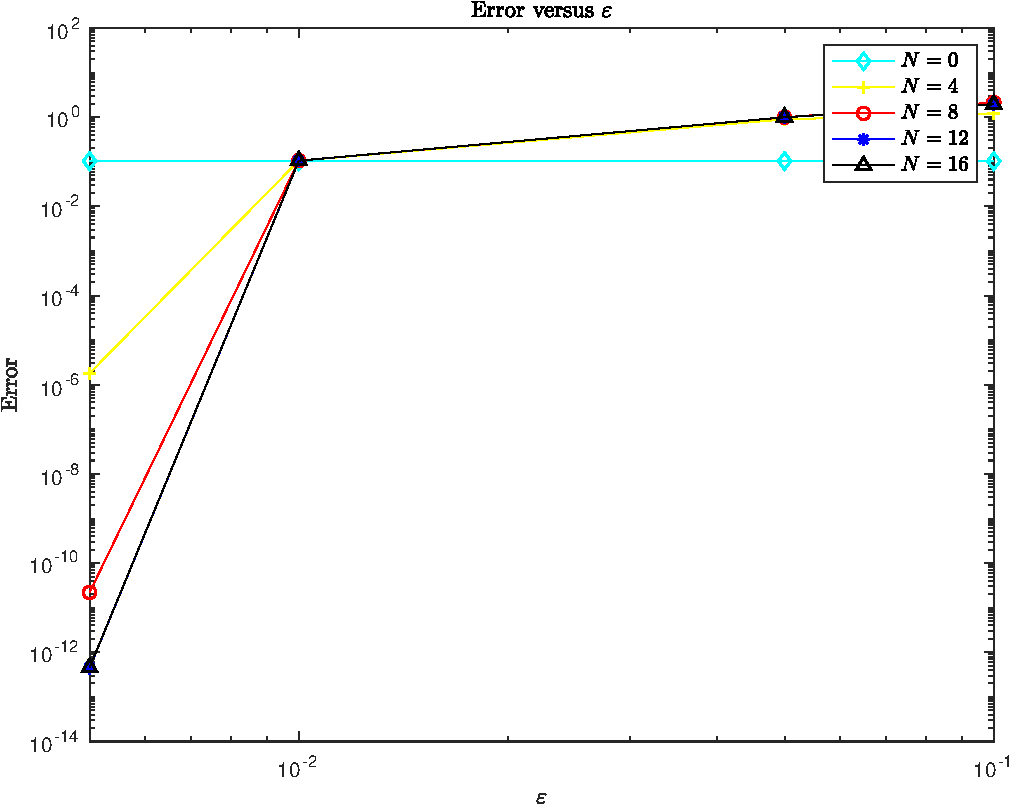
\includegraphics[width=0.4\textwidth]
		{fig_absErrrorVsEps_IIO_new.pdf}}
	\\
	\subfigure [new IIO with $a=1-10^{12}$.] 
	{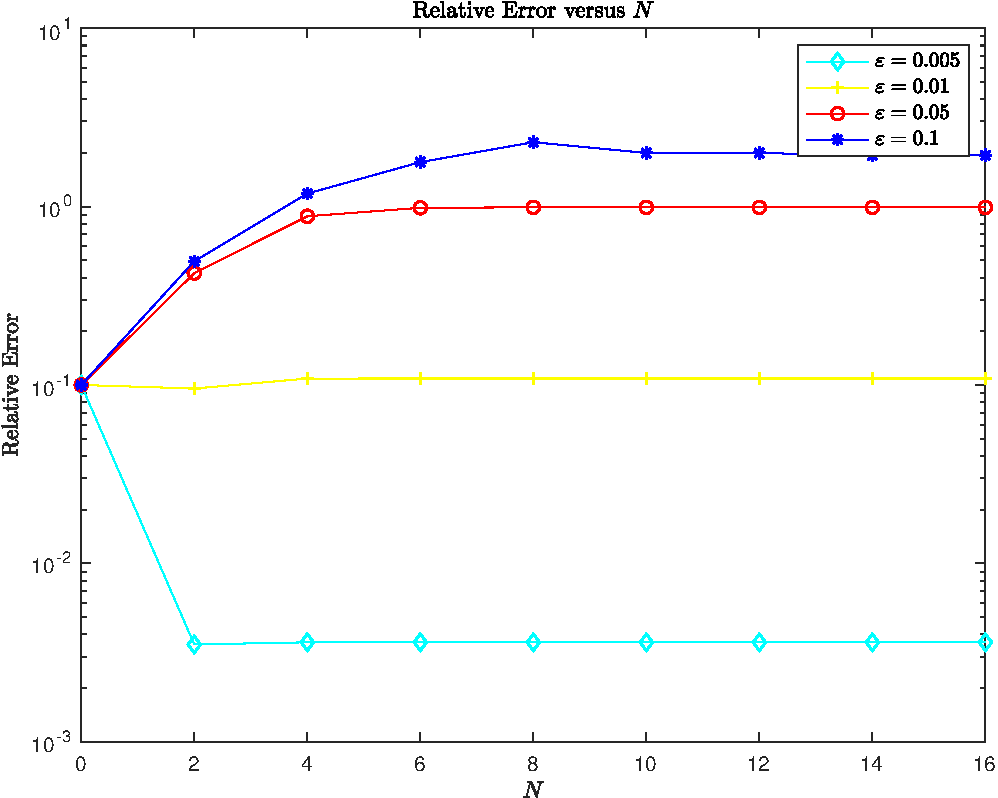
\includegraphics[width=0.4\textwidth]
		{fig_absErrrorVsN_IIO_new_sing12.pdf}}
	\quad
	\subfigure [new IIO with $a=1-10^{12}$.] 
	{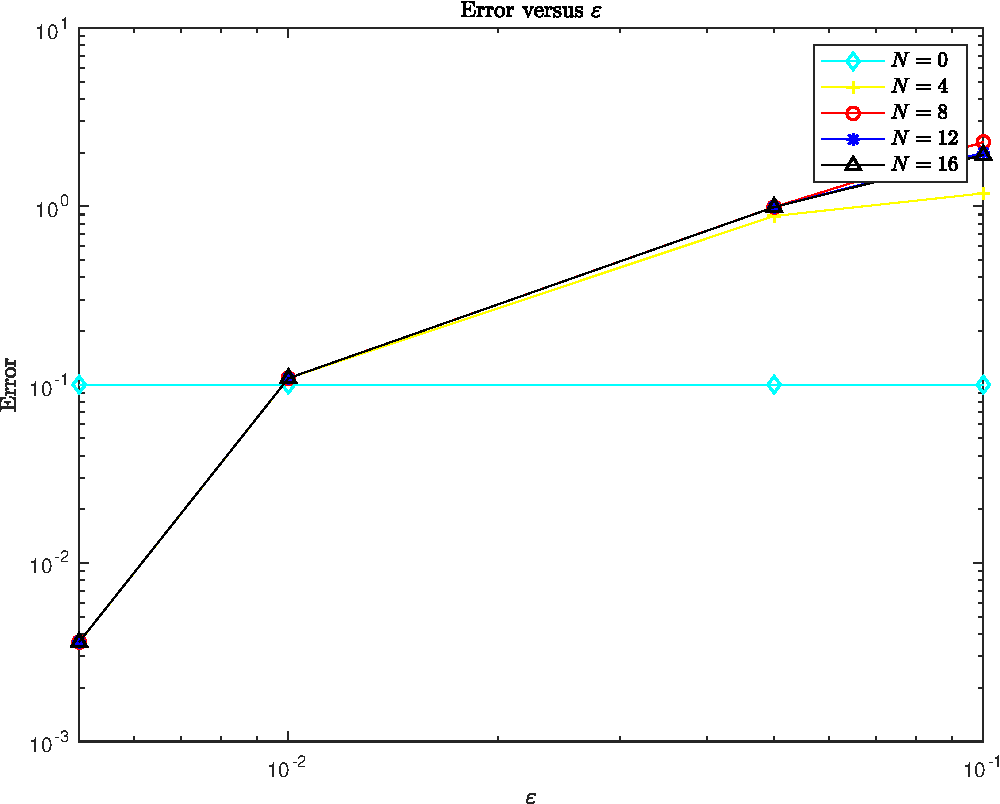
\includegraphics[width=0.4\textwidth]
		{fig_absErrrorVsEps_IIO_new_sing12.pdf}}
	\\
	\subfigure [new IIO with $a=1-10^{16}$.] 
	{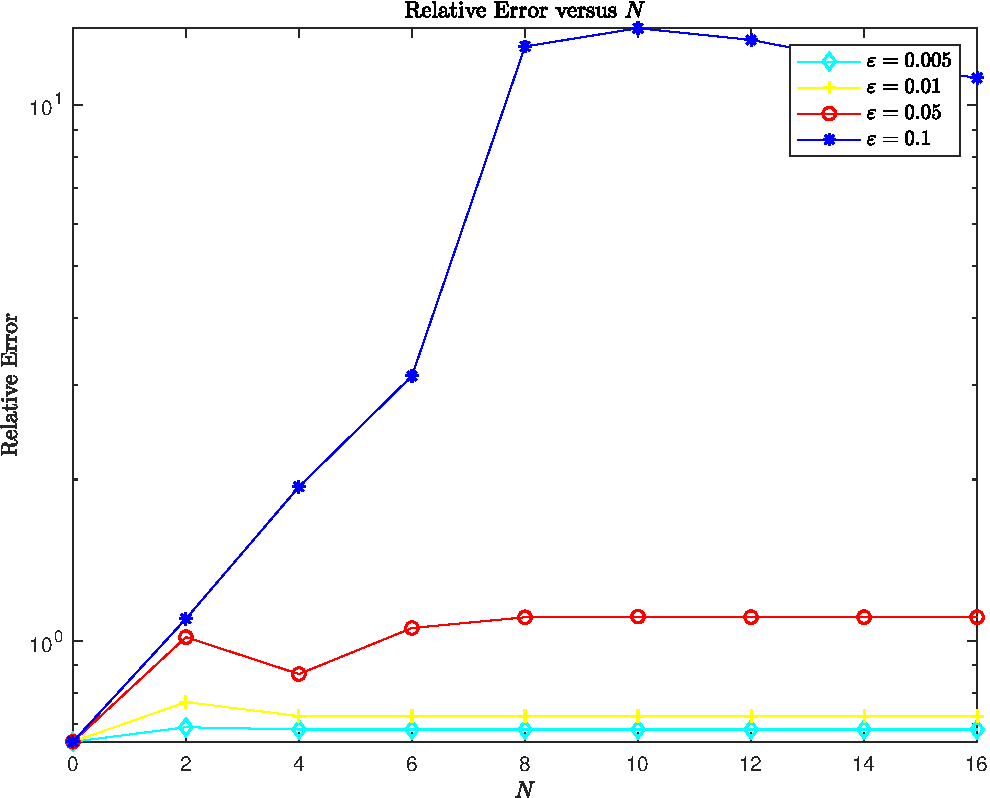
\includegraphics[width=0.4\textwidth]
		{fig_absErrrorVsN_IIO_new_sing16.pdf}}
	\quad
	\subfigure [new IIO with $a=1-10^{16}$.] 
	{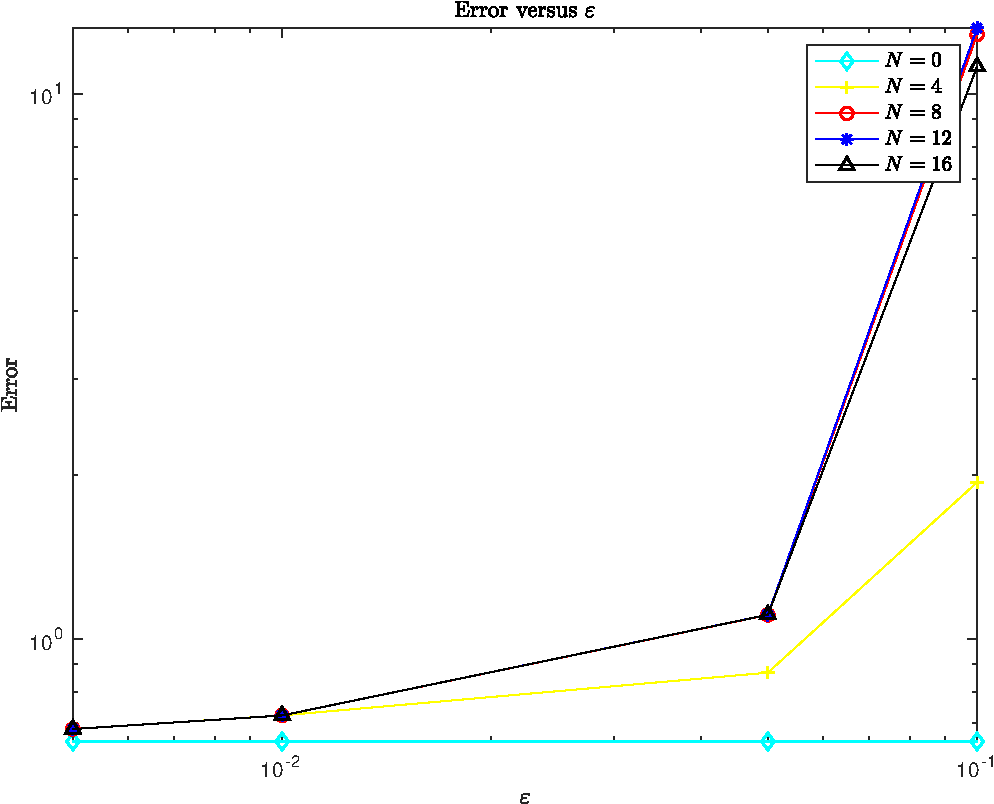
\includegraphics[width=0.4\textwidth]
		{fig_absErrrorVsEps_IIO_new_sing16.pdf}}
\end{figure}

\end{document}

